% Name: Cantor set
% Description: The first six steps of the Cantor set: start with a segment and keep removing the open middle third of every piece.
% Tags: Cantor set, fractal, middle thirds, measure zero

\usetikzlibrary{lindenmayersystems}

% F draws a piece and f skips a gap: each piece becomes piece, gap, piece, and each gap three gaps
\pgfdeclarelindenmayersystem{Cantor set}{
  \rule{F -> FfF}
  \rule{f -> fff}}

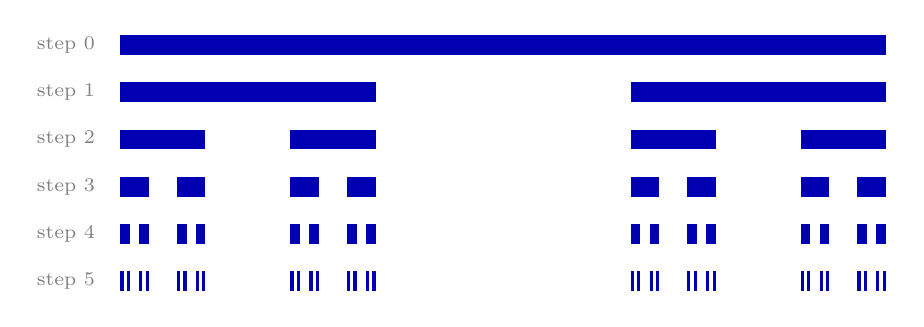
\begin{tikzpicture}
  \foreach \n in {0,...,5} {
    \pgfmathsetlengthmacro\st{9.72cm/3^\n}
    \draw[line width=2.5mm, blue!70!black, shift={(0,-0.6*\n)}, lindenmayer system={Cantor set, axiom=F, order=\n, step=\st}] lindenmayer system;
    \node[anchor=east, font=\scriptsize, gray] at (-0.2,-0.6*\n) {step \n};
  }
\end{tikzpicture}
